\documentclass[../main/main.tex]{subfiles}

\newdate{date}{09}{10}{2020}


\begin{document}

\begin{redbox}
\textbf{TO DO:} cercare di capire \textbf{accademicamente} il valore ottimale per la resistenza \( R_x \) per ottenere una potenza dissipata minore di \( 1 \times 10^{-4 } \) W.
Si ricorda che la potenza dissipata si può calcolare come:
\begin{equation*}
  P = \frac{V_B^2}{R_x} = V_{\text{gen}}^2 \frac{R_x}{(R_1+R_x)^2} < 1 \times 10^{-4} \text{ W}
\end{equation*}
e quindi
\begin{equation*}
  V_B^2 < \sqrt{R_x \times 10^{-4} }
\end{equation*}
\end{redbox}

\begin{greenbox}
\textbf{SOLUTION:} Non c'è una soluzione univoca. Con i valori precedentemente scelti otteniamo che:
\begin{equation*}
  P = V_{\text{gen}}^2 \frac{R_x}{(R_1+R_x)^2} = V_{\text{gen}}^2 \frac{28.8 \, \Omega }{(57.9 + 28.8)^2 \, \Omega^2}
  = V_{\text{gen}}^2 \times 3.83 \times 10^{-3} \, \Omega < 1 \times 10^{-4} \text{ W}
\end{equation*}
che implica:
\begin{equation*}
  V_{\text{gen}}^2 < 0.026  \longrightarrow V_{\text{gen}} < 0.16
\end{equation*}

La soluzione scelta alla fine è nel quaderno di Francesca (Prova-3).
\end{greenbox}

\begin{orangebox}
Per ridurre \( V_B = V_{\text{gen}} \frac{R_x}{(R_1+R_x)} \) bisogna o diminuire \( V_{\text{gen}} \) (aumenta l'errore sulla resistenza) oppure aumentare \( R_1 \).
\end{orangebox}

\subsection{Calibrazione AC}
Fatta la calibrazione in DC, si può passare a quella in \textbf{AC} utilizzando il generatore di segnali. In questo caso è necessario collegare la tensione utilizzando i cavi BNC-banana. Il bilanciamento si effettua con l'oscilloscopio. Vedere se il ponte funziona ancora e nel caso contrario capire il perché e cercare di trovare lo stesso risultato ottenuto con la calibrazione DC.

Sorge però un problema: siccome sia generatore che oscilloscopio hanno la massa a terra \( R_x \) è cortocircuitata (vedi Fig. \ref{fig:1}). Bisogna dunque aggiungere un trasformatore d'isolamento.

\marginpar{
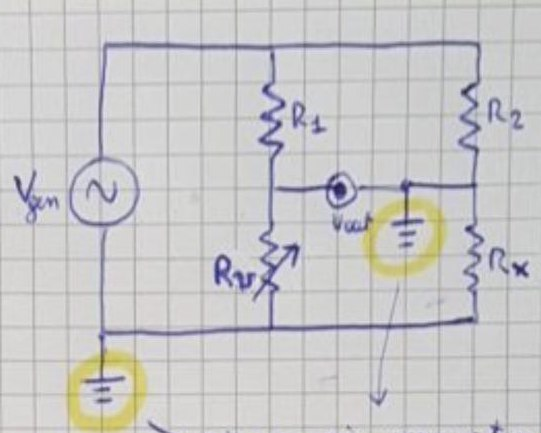
\includegraphics[width=\marginparwidth]{../lessons/image/02/1.jpg}
\captionof{figure}{\label{fig:1} \( R_x \) è cortocircuitata in AC.}
}


\marginpar{ \textbf{Laboratory 2.} \\  \displaydate{date}. \\ Compiled:  \today.}

Abbiamo cambiato le resistenze utilizzate per far quadrare il discorso della potenza dissipata. Abbiamo scelto:
\begin{equation*}
  R_1 = 15.01 \, \text{k} \Omega, \quad  R_2 = 14.89 \, \text{k} \Omega
\end{equation*}
Bisogna che disaccoppiamo i due circuiti (l'alimentazione e il ponte). Per fare ciò utilizziamo un trasformatore d'isolamento 1 a 1.

Inoltre, utilizzeremo l'amplificatore lock-in per ridurre il rumore. Infatti l'oscilloscopio rileva un range molto grande di frequenze, mentre il lock-in è settato solo sulla banda dei 30 Hz che sono di interesse.


\subsubsection{Problema resistenza dei fili}

Il termometro che utilizzeremo ha tre fili a cui verranno collegati 3 bnc. Questi fili sono resistivi in quanto devono essere inseriti all'interno del criostato e sono fatti di lega. Non possiamo utilizzare dei fili di rame (che hanno resistenza nulla) in quanto hanno un'alta conducibilità e non permetterebbero di raffreddare il superconduttore all'interno del criostato.

Adesso per simulare la resistenza dei fili utilizziamo delle resistenze di \( \sim 10 \, \Omega  \).

\begin{remark}
Lavoreremo range di temperatura di circa 80-90 K (il nostro superconduttore avrà una temperatura critica sui 90-100 K).
\end{remark}

\subsubsection{Configurazione finale}
Come configurazione finale del nostro circuito abbiamo scelto le resistenze \( R_1 \) e \( R_2 \), la resistenza \( R_x \equiv R_T \) e le resistenze parassiti dei fili come in Fig. \ref{fig:2_2}.

\begin{figure}[h!]
\centering
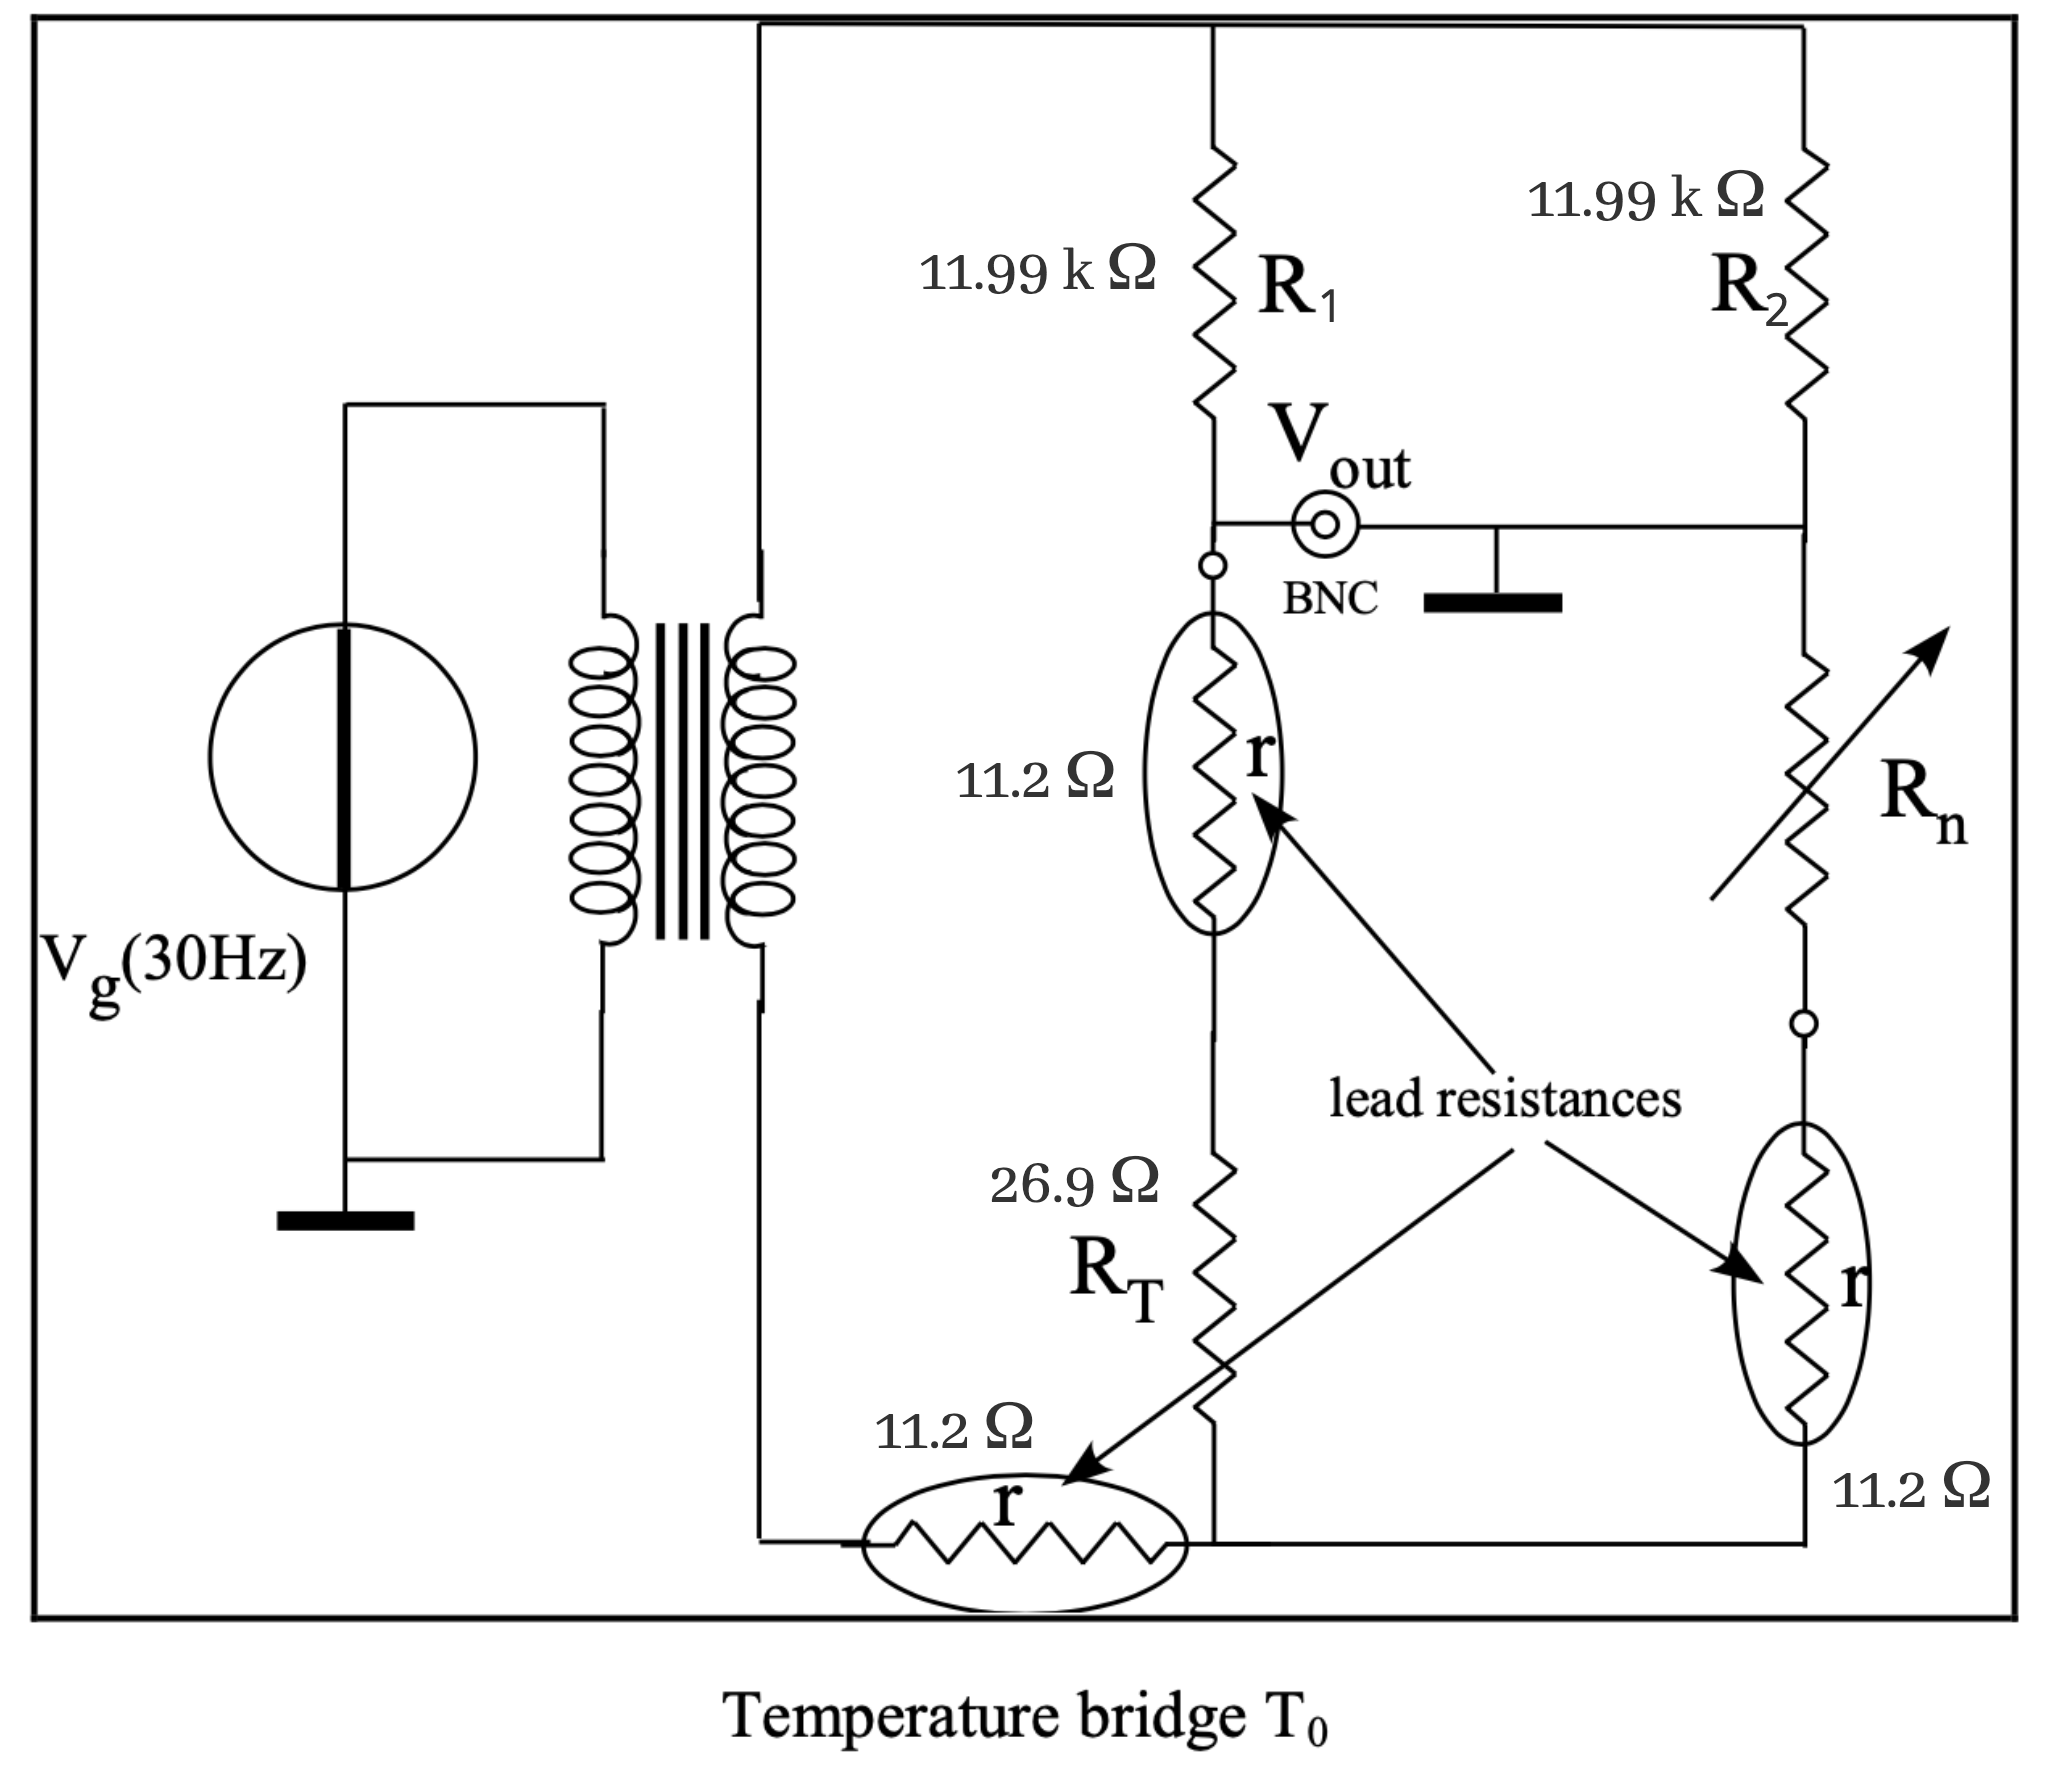
\includegraphics[width=0.8\textwidth]{../lessons/image/02/2.png}
\caption{\label{fig:2_2} Ponte di Wheatstone finale.}
\end{figure}








\end{document}
